\documentclass[11pt,a4paper]{article}

\usepackage[margin=2.3cm]{geometry}
\usepackage{amsmath,amssymb}
\usepackage{graphicx}
\usepackage{booktabs}
\usepackage{xcolor}
\usepackage{enumitem}
\usepackage[hidelinks]{hyperref}
\usepackage{caption}

\emergencystretch=1.5em
\captionsetup{font=small,labelfont=bf,width=.92\textwidth}
\setlength{\parskip}{4pt plus 1pt}
\setlength{\parindent}{0pt}

\newcommand{\code}[1]{\texttt{#1}}
\newcommand{\bst}[1]{\textbf{#1}}
\newcommand{\Kp}{K'}

\title{Soft forward, support-only value gradient\\[2pt]
\large Research note: does withholding the tail's value gradient recover the
hard-forward surrogate?}
\author{}
\date{2026-09-27.}

\begin{document}
\maketitle
\vspace{-2em}

% ============================================================
\section{Purpose and summary of conclusions}
% ============================================================

The soft-forward note (\code{docs/rblapsum-soft-forward.tex}) left a why open:
under the hard Top-$K$ evaluation, the soft-forward model loses badly to its
hard-forward twin, and one candidate explanation is training-signal dilution --
the optimizer trains all $K{+}J$ feature values at once instead of squeezing
the most out of the $K$ it will keep, as the hard-forward surrogate does. This
note tests that explanation directly. The regime
(\code{rblapsum\_sf\_value\_grad="support"}, ``sf-vsup'') keeps the soft
forward $y_i = z_i p_i$ over the pool unchanged, but the $J$ inactive
candidates receive no value gradient: only the score-path (support-change)
term reaches them, so their ranking still trains while their content does not.
Active features keep the soft value gradient $u\,p_i$; the boundary routing is
\code{through\_rank\_kappa} with support scale $1.0$, as everywhere.

If dilution were the mechanism, removing the tail's value training should
recover a substantial part of the hard-eval gap to the hard-forward twin. The
measured answer is that it recovers essentially none of it:

\begin{itemize}[leftmargin=1.4em]
\item \textbf{The hard-eval gap to the hard-forward twin persists in full.}
At the comparison step the gap is $+0.045$ to $+0.909$ nats across the grid --
the same magnitudes, the same growth with $J$, and the same inverse ordering
in $K$ as the unrestricted soft-forward family. Withholding the tail's value
gradient does not make the hardened model better.

\item \textbf{The ranking gradient alone still populates the tail.} The
trained forward carries $3$--$82$ units of probability mass beyond $K$
despite the tail's values never receiving task gradient: the score path by
itself moves tail features into the kernel's reach. The hard-eval damage
again tracks that mass within each $K$.

\item \textbf{Tail value training was a small benefit, not a cost.} Under
soft evaluation sf-vsup is slightly \emph{worse} than the unrestricted soft
forward in every directly comparable cell ($+0.010$ to $+0.024$ nats), while
still beating the pool-matched hard Top-$\Kp$ baseline everywhere
($-0.059$ to $-0.103$).

\item \textbf{Instability is unchanged, placing it in the score path.}
$(128,128)$ at $T=2$ diverged at step 3520; the unrestricted soft forward
died at 3480 in the same cell, and the hard-forward twin survives it. The
value-gradient mask is irrelevant to the divergence, consistent with the
boundary-mechanism analysis of the kappa-ablation note.

\item \textbf{One local exception.} At the two largest-$K$ $T=2$ cells the
mask reduces the late hard-eval drift the unrestricted family shows:
$(256,256)$ ends $0.222$ and $(128,384)$ $0.109$ nats better than sf at the
same step, both still far above kappa. An observation about two cells, not a
mechanism.
\end{itemize}

Taken together: the hard-eval loss of the soft forward is carried by the
forward-context mismatch itself -- the model is trained with weighted tails
present and evaluated with them deleted -- and not by where the value
gradient goes.

% ============================================================
\section{Setup}
% ============================================================

Twenty runs, identical to the soft-forward campaign in every respect but two.
The ten $(K,J)$ cells and both variants ($T=2$; post-norm at $T=1$) inherit
the same hard-forward twins' \code{config.json} files with the mode fields
overridden, on the same machine and repo state
(\code{rblapsum\_sf\_value\_grad="support"} added in commit \code{1dd3764}).
First, the value-gradient mask above. Second, the horizon: the runs stop at
10k of the configured 20k steps, with \code{max\_steps} -- and with it the
learning-rate cosine and every schedule -- untouched
(\code{train\_guard --stop-step}), so the trajectory up to the stop is
step-for-step comparable with the full-length references. All comparisons in
this note are therefore read at \textbf{step 9500}, the last validation step
common to every run: the stop fires on the step-10000 training log, which
precedes that step's validation pass in twelve of the twenty runs.

References, both at their own step-9500 points: the hard-forward
\code{through\_rank\_kappa} twins, and the five hard Top-$\Kp$ post-norm
baselines. Metrics as before: \code{val/ce} is the hard Top-$K$ forward,
\code{val\_soft/ce} the trained soft forward, \code{rb\_soft\_mass} the
pool's probability mass $\sum_i p_i$.

% ============================================================
\section{Results}
% ============================================================

\subsection*{Hard evaluation}

\code{val/ce} at step 9500, sf-vsup against its hard-forward twin:

\begin{center}\small
\begin{tabular}{lcccccc}
\toprule
& \multicolumn{3}{c}{$T=2$} & \multicolumn{3}{c}{post-norm} \\
\cmidrule(lr){2-4}\cmidrule(lr){5-7}
$(K,J)$ & kappa & sf-vsup & gap & kappa & sf-vsup & gap \\
\midrule
$(32,32)$   & 1.6758 & 1.7470 & $+0.071$ & 1.6591 & 1.7590 & $+0.100$ \\
$(32,96)$   & 1.6374 & 1.9294 & $+0.292$ & 1.6389 & 1.8749 & $+0.236$ \\
$(32,224)$  & 1.6114 & 2.1871 & $+0.576$ & 1.6211 & 2.0758 & $+0.455$ \\
$(32,480)$  & 1.6218 & 2.5308 & $+0.909$ & 1.6717 & 2.2258 & $+0.554$ \\
$(64,64)$   & 1.6403 & 1.6967 & $+0.056$ & 1.6077 & 1.6839 & $+0.076$ \\
$(64,192)$  & 1.6156 & 1.8370 & $+0.221$ & 1.5822 & 1.7880 & $+0.206$ \\
$(64,448)$  & 1.6006 & 2.0097 & $+0.409$ & 1.5773 & 1.9270 & $+0.350$ \\
$(128,128)$ & 1.6117 & \multicolumn{2}{c}{diverged (3520)} & 1.5700 & 1.6239 & $+0.054$ \\
$(128,384)$ & 1.5874 & 1.7647 & $+0.177$ & 1.5556 & 1.7286 & $+0.173$ \\
$(256,256)$ & 1.5773 & 1.6809 & $+0.104$ & 1.5442 & 1.5891 & $+0.045$ \\
\bottomrule
\end{tabular}
\end{center}

The pattern of the soft-forward note is reproduced unchanged: the loss grows
with $J$ at every $K$, shrinks with $K$, and the post-norm is less damaged
than $T=2$ at wide windows. Masking the tail's value gradient has not moved
it.

\subsection*{Soft evaluation}

\code{val\_soft/ce} at step 9500, grouped by pool, against hard Top-$\Kp$
at the same step:

\begin{center}\small
\begin{tabular}{llcccc}
\toprule
pool $\Kp$ & $(K,J)$ & sf-vsup $T{=}2$ & sf-vsup post-norm & hard Top-$\Kp$ & best margin \\
\midrule
$64$  & $(32,32)$   & \bst{1.5690} & 1.6049 & 1.6718 & $-0.103$ \\
\midrule
$128$ & $(32,96)$   & 1.5356 & 1.5530 & 1.6267 & $-0.091$ \\
      & $(64,64)$   & \bst{1.5351} & 1.5470 & & $-0.092$ \\
\midrule
$256$ & $(32,224)$  & 1.5193 & 1.5312 & 1.5928 & $-0.074$ \\
      & $(64,192)$  & \bst{1.5099} & 1.5214 & & $-0.083$ \\
      & $(128,128)$ & --- & 1.5152 & & $-0.078$ \\
\midrule
$512$ & $(32,480)$  & \bst{1.5009} & 1.5224 & 1.5597 & $-0.059$ \\
      & $(64,448)$  & 1.5027 & 1.5080 & & $-0.057$ \\
      & $(128,384)$ & 1.5104 & 1.5032 & & $-0.056$ \\
      & $(256,256)$ & 1.5137 & 1.5095 & & $-0.050$ \\
\bottomrule
\end{tabular}
\end{center}

Every cell still beats the pool-matched hard baseline, $T=2$ still leads the
post-norm almost everywhere, widening $J$ still helps monotonically, and $K$
still barely matters at fixed pool -- the soft-evaluation regularities of the
unrestricted family survive the mask intact.

\subsection*{Against the unrestricted soft forward}

At step 9500, sf-vsup minus sf, same cell and variant (positive = the mask
hurt):

\begin{center}\small
\begin{tabular}{lcccc}
\toprule
& \multicolumn{2}{c}{hard eval} & \multicolumn{2}{c}{soft eval} \\
\cmidrule(lr){2-3}\cmidrule(lr){4-5}
$(K,J)$ & $T{=}2$ & post-norm & $T{=}2$ & post-norm \\
\midrule
$(32,32)$   & $-0.014$ & $+0.015$ & $+0.011$ & $+0.024$ \\
$(32,96)$   & $-0.008$ & $+0.011$ & $+0.018$ & $+0.016$ \\
$(32,224)$  & $+0.039$ & $+0.091$ & $+0.023$ & $+0.008$ \\
$(32,480)$  & $+0.158$ & $+0.191$ & $+0.015$ & $+0.005$ \\
$(64,64)$   & $-0.022$ & $+0.005$ & $+0.010$ & $+0.013$ \\
$(64,192)$  & $-0.034$ & $+0.012$ & $+0.009$ & $+0.018$ \\
$(64,448)$  & $-0.015$ & $+0.055$ & $+0.023$ & $+0.012$ \\
$(128,128)$ & --- & $+0.003$ & --- & $+0.008$ \\
$(128,384)$ & $-0.109$ & $+0.013$ & $-0.051$ & $+0.009$ \\
$(256,256)$ & $-0.222$ & $+0.005$ & $+0.016$ & $+0.008$ \\
\bottomrule
\end{tabular}
\end{center}

Three readings. Under soft evaluation the mask costs a small, uniform amount
($+0.008$ to $+0.024$; the one negative entry is the window of sf's recovered
excursion at $(128,384)$, $T=2$, which contaminates the sf reference there) --
the tail's value training was contributing quality, not diluting it. Under
hard evaluation the differences are small and two-signed at $J \le 3K$, and
the mask clearly \emph{hurts} at the widest $K=32$ windows. The two large
negative entries ($T=2$ at $(256,256)$ and $(128,384)$) are the late-drift
exception flagged in the summary.

\subsection*{Tail mass without tail value training}

\code{rb\_soft\_mass} $-\,K$ at the end of each run:

\begin{center}\small
\begin{tabular}{lcc|lcc}
\toprule
$(K,J)$ & $T{=}2$ & post-norm & $(K,J)$ & $T{=}2$ & post-norm \\
\midrule
$(32,32)$  & 3.9  & 2.9  & $(64,448)$  & 81.5 & 29.4 \\
$(32,96)$  & 15.8 & 8.2  & $(128,128)$ & ---  & 9.0  \\
$(32,224)$ & 35.2 & 16.3 & $(128,384)$ & 75.6 & 27.4 \\
$(32,480)$ & 72.3 & 27.9 & $(256,256)$ & 23.5 & 15.3 \\
$(64,64)$  & 7.7  & 5.2  & & & \\
\bottomrule
\end{tabular}
\end{center}

The tails carry substantial mass even though their values receive no task
gradient: the score path alone -- the ranking signal, including the
$\kappa$-distributed boundary term -- moves inactive features into the
kernel's reach, and the hard-eval gap again grows with this mass within each
$K$. This is the mechanical reason the mask cannot close the gap: the
forward's tail contribution, which hard evaluation deletes, is built by the
part of the gradient the mask keeps.

\subsection*{Stability}

$(128,128)$ at $T=2$ diverged at step 3520 (best CE $1.72$, then the
gradient-norm blowup; guard ceiling rule), against 3480 for the unrestricted
soft forward and survival for the hard-forward twin. The value-gradient mask
neither delays nor prevents the divergence, so the instability is carried by
the score path. All other cells reached the horizon; no recovered excursions
this time.

\subsection*{Figures}

Layout as in the soft-forward note: per pool, left $T=2$, right post-norm;
hard-forward twins in blues, sf-vsup in oranges (light to dark with $K$),
hard Top-$\Kp$ dashed black; vertical axis the hard-eval \code{val/ce}; the
horizon is 10k steps. The soft-eval figure repeats \code{val\_soft/ce} for
the sf-vsup family against the same ladder.

\begin{figure}[htb]\centering
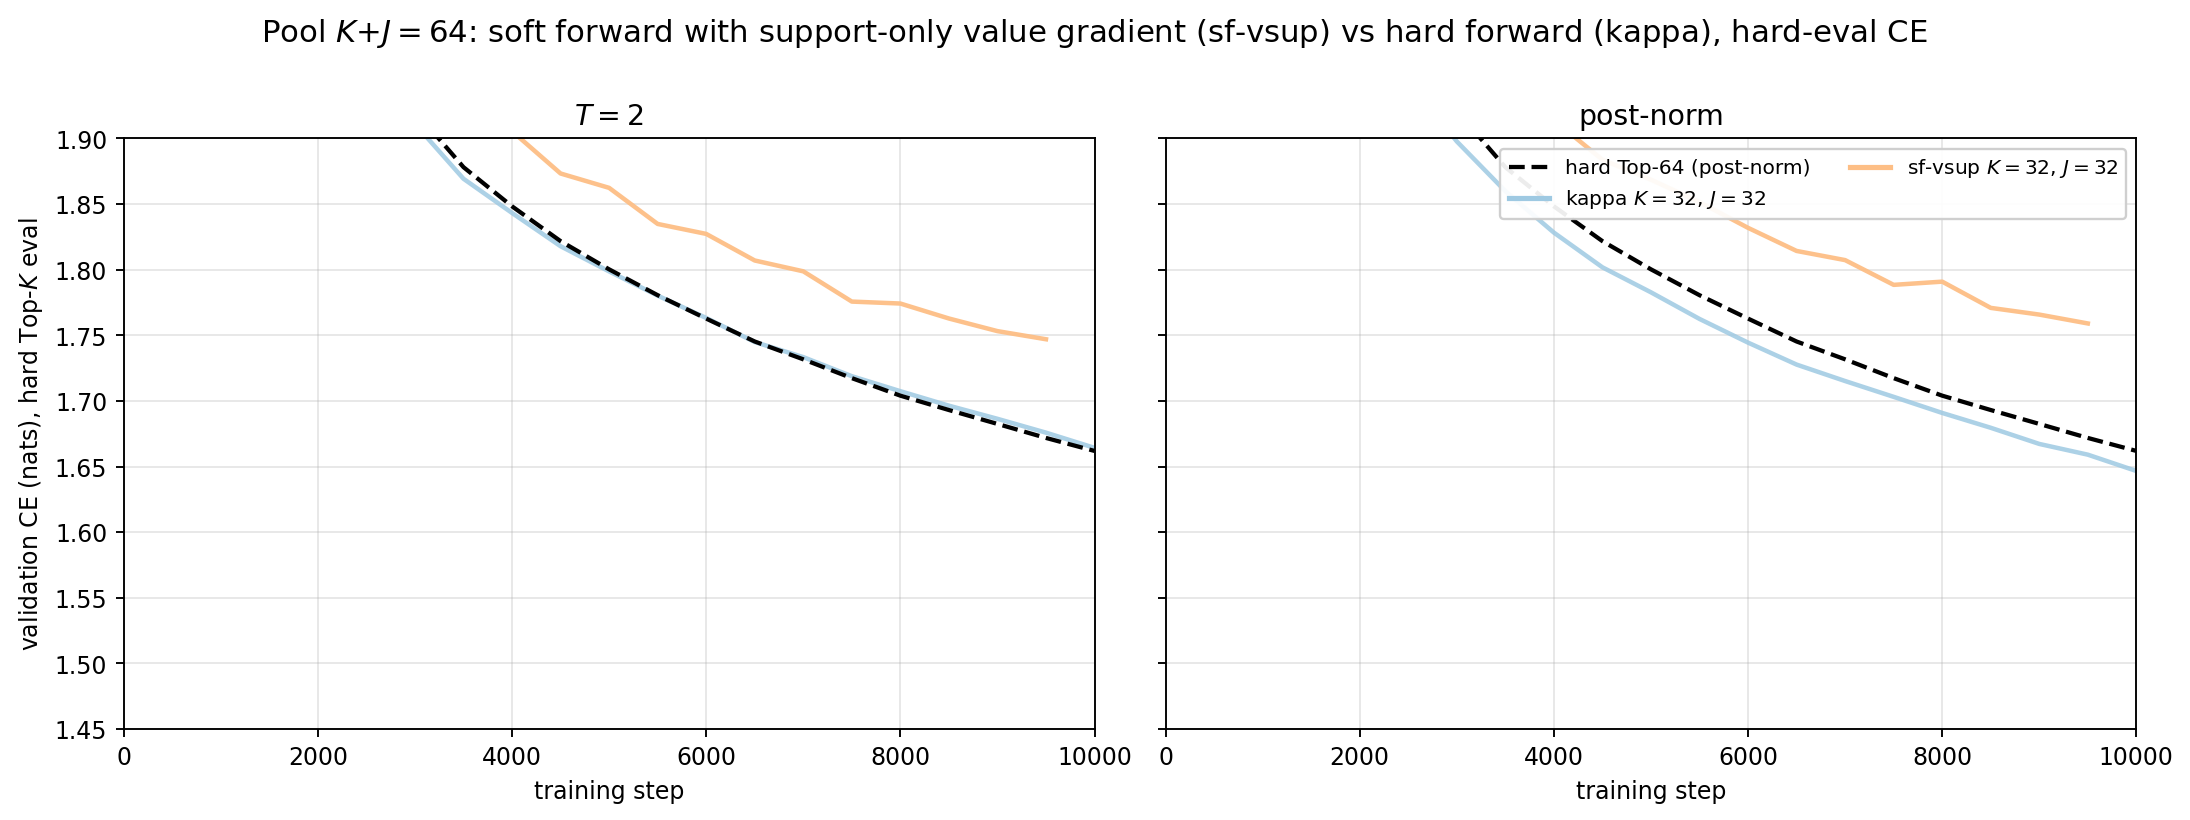
\includegraphics[width=\textwidth]{figures/sfv/sfv_pool_k64.png}
\caption{Pool $\Kp=64$. The single cell $(32,32)$ sits $0.07$--$0.10$ nats
above its twin under hard eval -- the same offset the unrestricted soft
forward shows here.}
\end{figure}

\begin{figure}[htb]\centering
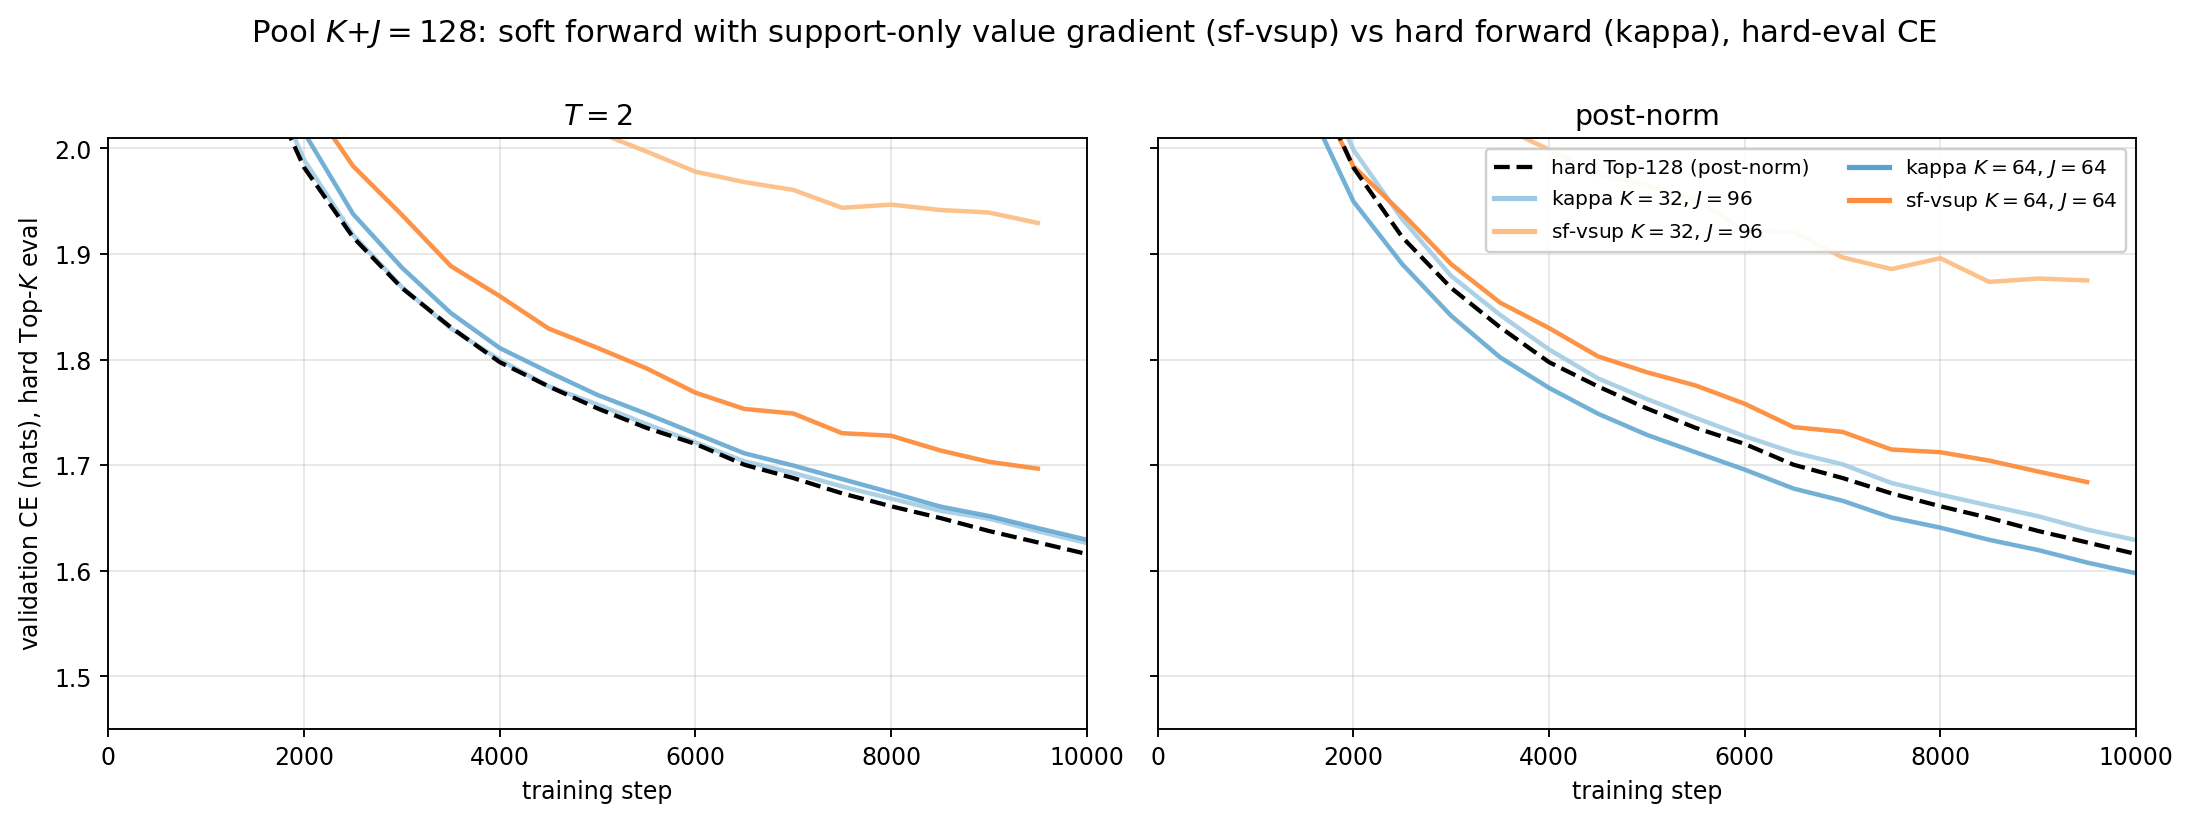
\includegraphics[width=\textwidth]{figures/sfv/sfv_pool_k128.png}
\caption{Pool $\Kp=128$. Both cells trail their twins by $0.06$--$0.24$
nats; the ordering and the $J$-dependence match the unrestricted family.}
\end{figure}

\begin{figure}[htb]\centering
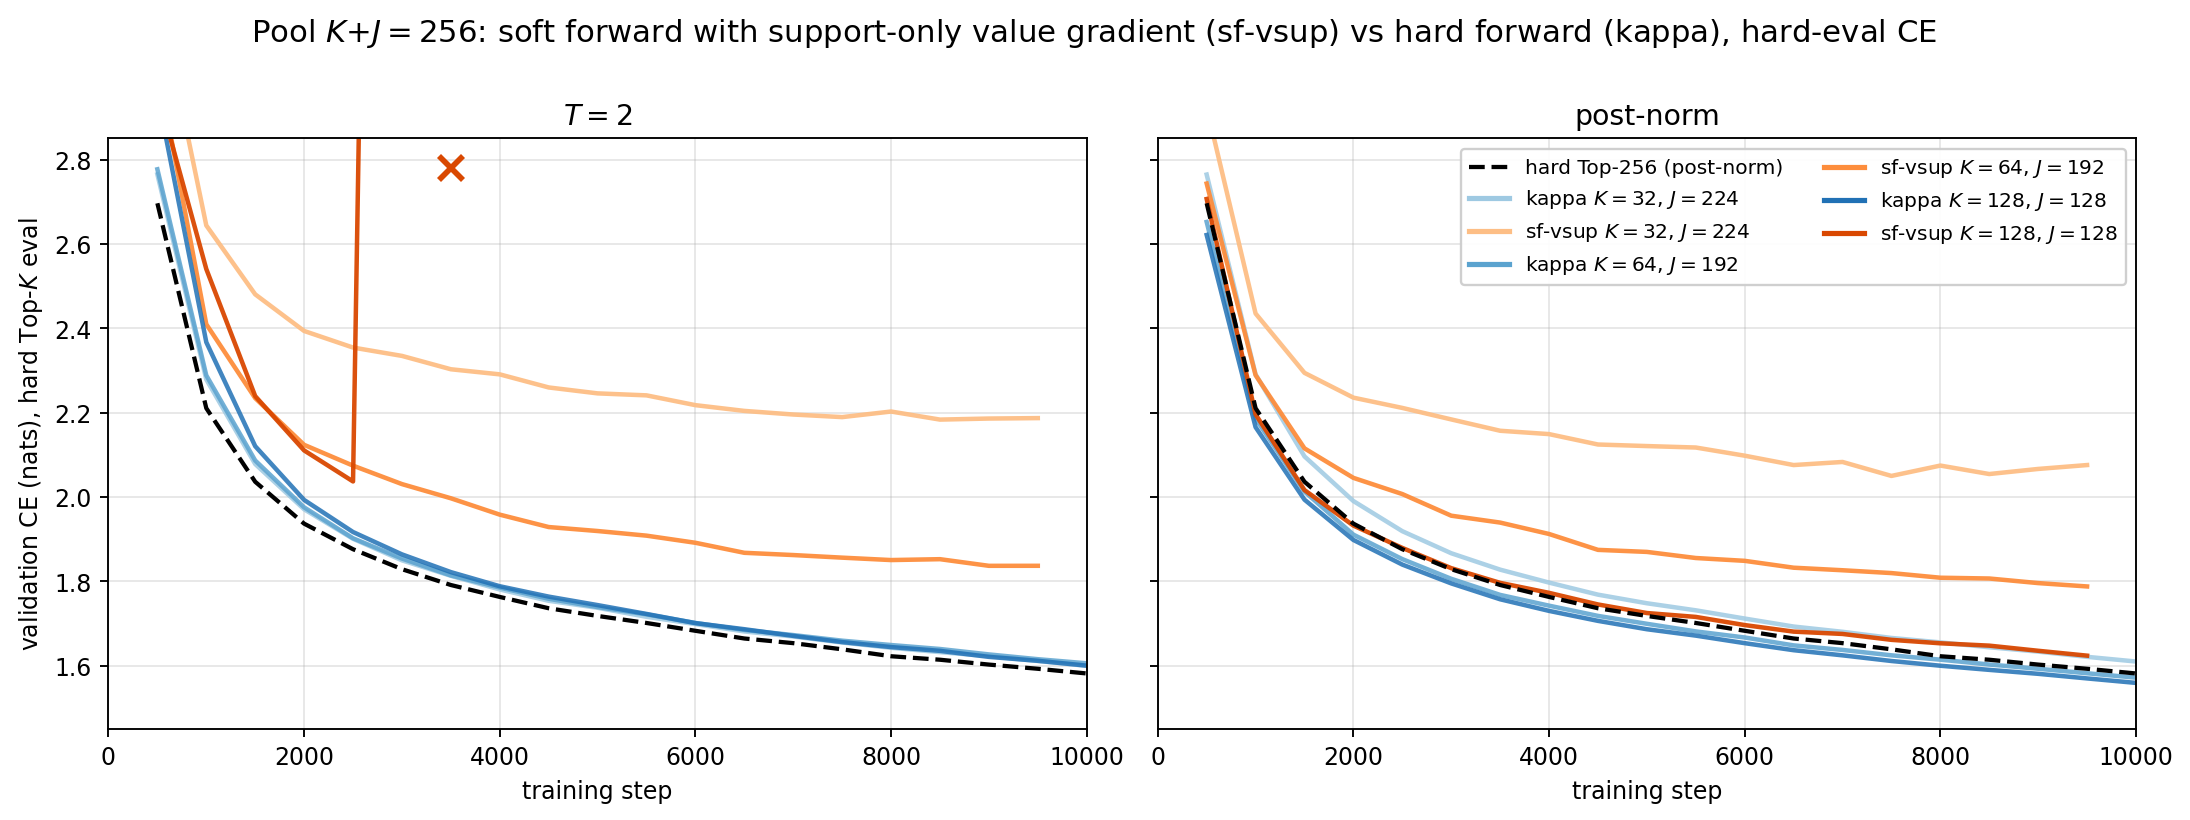
\includegraphics[width=\textwidth]{figures/sfv/sfv_pool_k256.png}
\caption{Pool $\Kp=256$. The $T=2$ cell at $(128,128)$ ends at its guard
stop (cross), the second soft-forward death of this cell at 3.5k steps.}
\end{figure}

\begin{figure}[htb]\centering
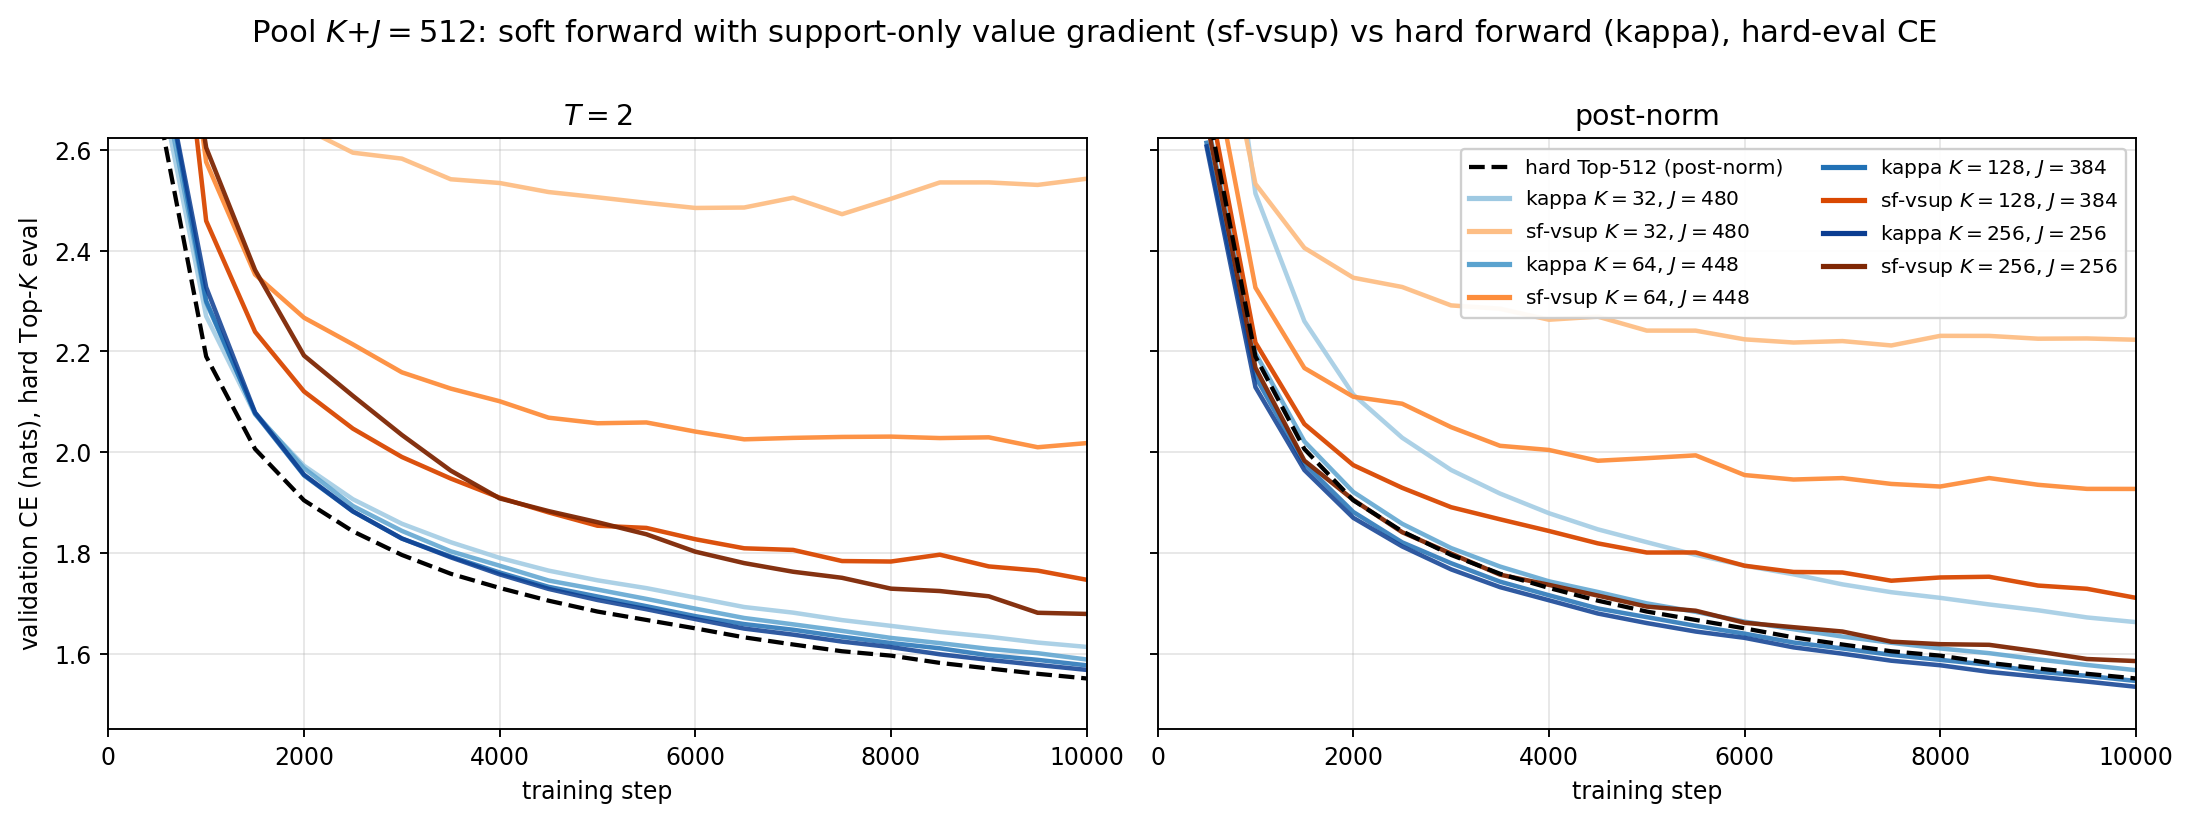
\includegraphics[width=\textwidth]{figures/sfv/sfv_pool_k512.png}
\caption{Pool $\Kp=512$. The widest windows: the orange family sits
$0.05$--$0.9$ nats above the blues under hard eval. Unlike the unrestricted
soft forward, the $T=2$ cells at $K=128$ and $256$ do not drift upward late
-- the one visible effect of the value-gradient mask.}
\end{figure}

\begin{figure}[htb]\centering
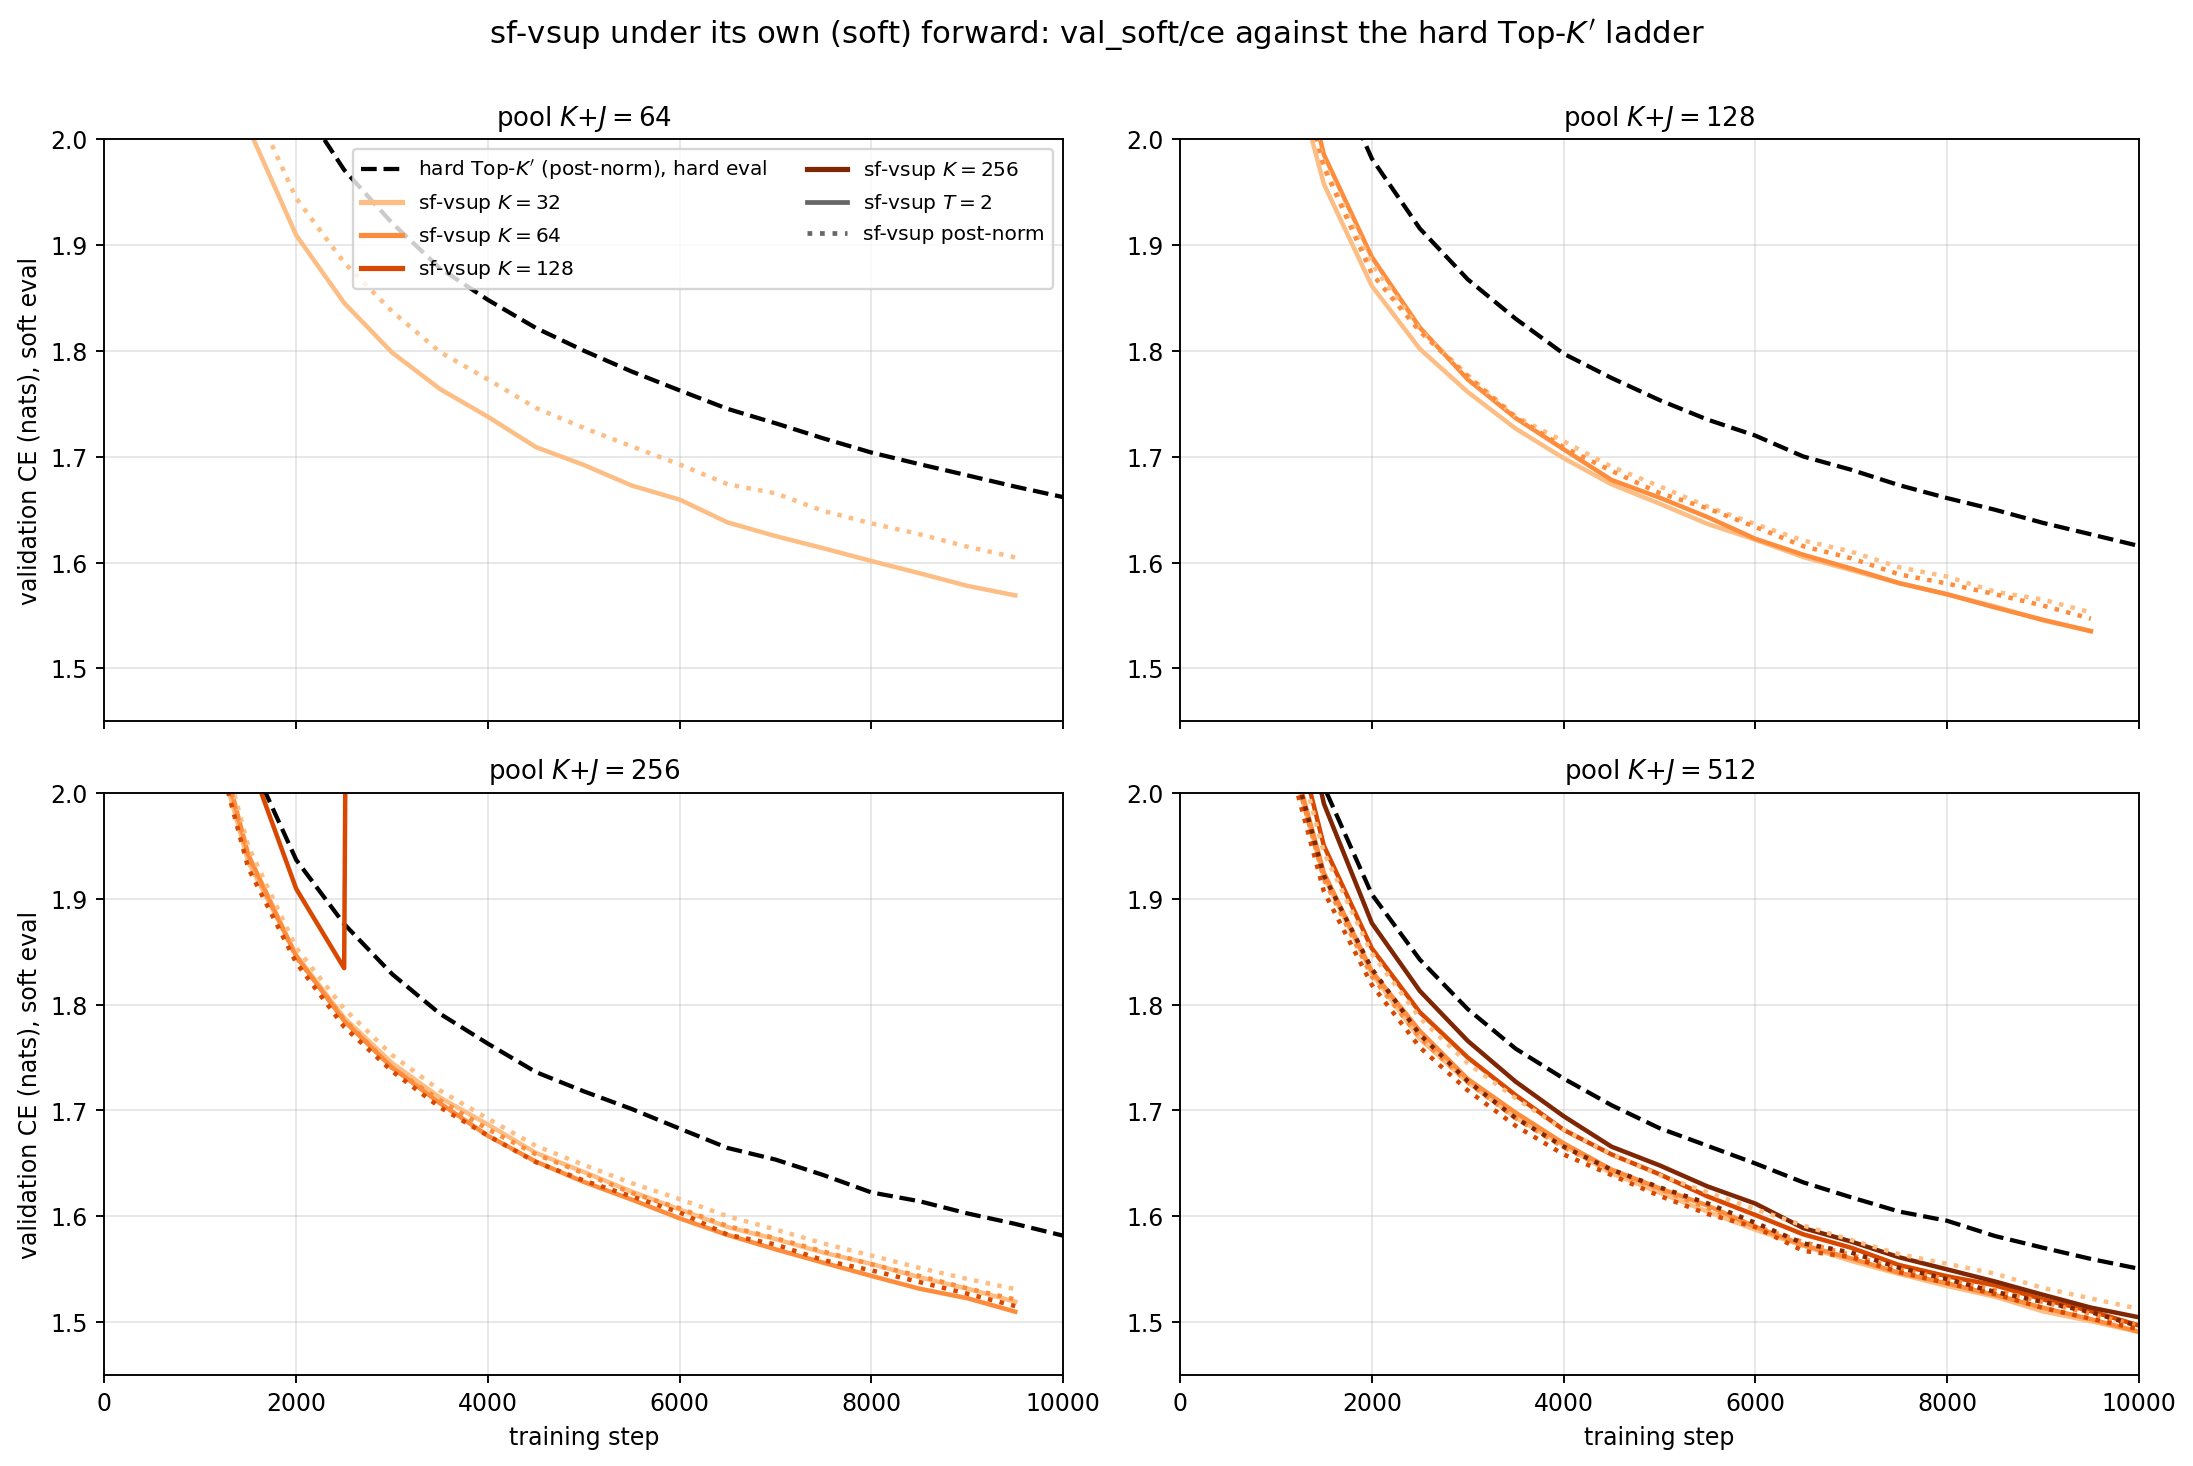
\includegraphics[width=\textwidth]{figures/sfv/sfv_soft_eval.png}
\caption{sf-vsup under its own forward (\code{val\_soft/ce}), per pool,
against the pool-matched hard Top-$\Kp$ baseline (dashed). Solid $T=2$,
dotted post-norm. Every curve ends below the dashed reference; the cluster
across $K$ is tight, as in the unrestricted family.}
\end{figure}

% ============================================================
\section{Interpretation}
% ============================================================

The experiment separates two explanations the soft-forward note could not:
that the soft forward's hard-eval loss comes from diluting the training
signal across $K{+}J$ feature values, or from the forward-context mismatch --
active features are trained in the presence of weighted tails that hard
evaluation then deletes. Removing the tail's value gradient eliminates the
dilution channel by construction, and the hard-eval gap does not move. The
mismatch explanation is left carrying the result, and the tail-mass table
shows why it must: the ranking signal alone rebuilds the tail contribution,
so the trained forward still depends on features the hard forward drops.

The mask's measurable effects are all second-order and both-signed. It costs
a small uniform amount of soft-eval quality (the tail values were learning
something useful), it hurts hard eval at small $K$ with very wide windows
(with only the ranking signal, the tail that does form is less coordinated
with the actives, and at $K=32$, $J=480$ the forward leans on it heavily),
and it damps the late hard-eval drift of the two largest-$K$ $T=2$ cells.
None of this changes any conclusion of the soft-forward note.

For the programme, the negative result is the useful part: closing the
train/inference gap is not a matter of where the value gradient goes. The
remaining levers are the ones named before -- annealing $T$ toward a hard
forward, a hardening fine-tune, or a penalty on \code{rb\_soft\_mass} -- all
of which act on the forward's tail mass itself rather than on the gradient's
routing.

% ============================================================
\section{Scope}
% ============================================================

Single runs at one seed, and a 10k-step horizon on the 20k schedule: all
numbers are mid-training values at step 9500, directly comparable across
families because every run shares the schedule, but not comparable with the
20k finals of the earlier notes. The unrestricted-sf comparison reuses that
campaign's runs at the same step and machine. The hard-forward references
remain the retired machine's runs. The $(128,384)$, $T=2$ sf reference at
step 9500 sits inside that run's recovered excursion, so the one cell where
the mask appears to help soft eval is an artifact of the reference, not of
the mask. Only \code{through\_rank\_kappa} at support scale $1.0$ was
trained, and the mask was tested only at the two extremes (all pool values
train, or only the support's); a fractional version was not run.

\end{document}
